\documentclass{article}
\usepackage{amsmath}
\usepackage{amssymb}
\usepackage{enumitem}
\usepackage{algorithm}
\usepackage{listings}
\usepackage{color,xcolor}
\usepackage[T1]{fontenc}
\usepackage{etoolbox}
\usepackage{multicol}
\usepackage{geometry}
\usepackage{tikz, pgfplots, tkz-euclide,calc}
    \usetikzlibrary{patterns,snakes,shapes.arrows,3d}
    \geometry{
        total = {160mm, 237mm},
        left = 25mm,
        right = 35mm,
        top = 30mm,
        bottom = 30mm,
      }

\newcommand{\enter}{\raisebox{-1.8pt}{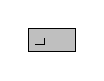
\begin{tikzpicture}[scale=0.3]
    \draw[thin,fill=lightgray] (0,0) rectangle (2,1);
    \draw (0.3,0.3) -- (0.7,0.3)--(0.7,0.6);     
\end{tikzpicture}}}

\definecolor{pgray}{rgb}{0.5,0.5,0.5}
\definecolor{pblue}{rgb}{0.13,0.13,1}
\definecolor{pgreen}{rgb}{0,0.5,0}
\definecolor{pred}{rgb}{0.9,0,0}
\definecolor{pgrey}{rgb}{0.46,0.45,0.48}
\definecolor{pcyan}{HTML}{D4EFFC}
\definecolor{lblue}{HTML}{00AEEF}
\definecolor{input}{HTML}{AAE1FA}
\definecolor{bg}{rgb}{0.95, 0.95, 0.92}
\definecolor{vscode}{HTML}{282A36}

\newcommand{\nextline}[1]{\raisebox{0pt}[1pt]{\colorbox{input}{#1}}}

\usepackage{listings}
\lstset{language=Java,
  showspaces=false,
  showtabs=false,
  breaklines=true,
  showstringspaces=false,
  breakatwhitespace=true,
  commentstyle=\color{pgray},
  keywordstyle=\color{pblue},
  stringstyle=\color{pgreen},
  basicstyle=\small\ttfamily,
  frame=single,
  backgroundcolor=\color{pcyan},
  escapeinside={(*}{*)},
}
\newcommand{\jawab}{\textbf{Solve}:}

\begin{document}
    \pagenumbering{gobble}
    \setcounter{section}{3}
    \setcounter{subsection}{1}
    \begin{tabular}{|lcl|}
     \hline
     Nama&:&Teosofi Hidayah Agung\\
     NRP&:&5002221132\\
     \hline
    \end{tabular}

    \begin{enumerate}
        \item[\color{lblue}11.4] (\textit{Maximum element in} \texttt{\color{lblue}ArrayList}) Write the following method that returns the maximum value in an \texttt{\color{lblue}ArrayList} of integers. The method returns \texttt{\color{lblue}null} if the list is null or the list size is {\color{lblue}0}.
        \begin{lstlisting}[frame=none,backgroundcolor=]
public static Integer max(ArrayList<Integer> list)
        \end{lstlisting}
        \jawab\\
        The method can be implemented as follows:
        \begin{lstlisting}[backgroundcolor=\color{bg}]
public static Integer max(ArrayList<Integer> list) {
    if (list == null || list.size() == 0) return null;
    Integer max = list.get(0);
    for (int i = 1; i < list.size(); i++) {
        if (list.get(i) > max) max = list.get(i);
    }
    return max;
}
        \end{lstlisting}
        \texttt{Integer} is used instead of \texttt{int} to allow the method to return \texttt{null} if the list is null or empty.

        \item[\color{lblue}11.9] (\textit{Largest row and column}) Write a program that randomly fills in {\color{lblue}0}s and {\color{lblue}1}s into a n-by-n matrix, prints the matrix, and finds the rows and columns with the most {\color{lblue}1}s. (Hint: Use two {\color{lblue} ArrayLists} to store the row and column indices with the most {\color{lblue}1}s.) Here is a sample run of the program:
        \begin{lstlisting}
Enter the array size n: (*\nextline{4}*) (*\enter*)
The random array is
0011
0011
1101
1010
The largest row index: 2
The largest column index: 2, 3
        \end{lstlisting}
        \jawab\\
        Index of row and coloumn it's start from zero. First, we create all the necessary method as follows:
        \begin{lstlisting}[backgroundcolor=\color{bg}]
package Aplro2.Week14;

import java.util.ArrayList;
import java.util.Random;

public class Liang_Ch11_9 {
    // Create a n-by-n matrix filled with random 0s and 1s
    public static ArrayList<ArrayList<Integer>> rMatrix(int size) {
        Random random = new Random();
        ArrayList<ArrayList<Integer>> list = new ArrayList<>();
        for (int i = 0; i < size; i++) {
            ArrayList<Integer> innerList = new ArrayList<>();
            for (int j = 0; j < size; j++) {
                innerList.add(random.nextInt(2));
            }
            list.add(innerList);
        }
        return list;
        \end{lstlisting}
        \begin{lstlisting}[backgroundcolor=\color{bg}]
    }
    // Return the Row index with the most 1s
    public static ArrayList<ArrayList<Integer>> MaxRowCol(ArrayList<ArrayList<Integer>> list) {
        ArrayList<ArrayList<Integer>> result = new ArrayList<>();
        ArrayList<Integer> maxRow = new ArrayList<>();
        ArrayList<Integer> maxCol = new ArrayList<>();
        int maxR = 0;
        int maxC = 0;
        for (int i = 0; i < list.size(); i++) {
            int sumR = 0;
            int sumC = 0;
            for (int j = 0; j < list.get(i).size(); j++) {
                sumR += list.get(i).get(j);
                sumC += list.get(j).get(i);
            }
            //Check Row
            if (sumR > maxR) {
                maxR = sumR;
                maxRow.clear();
                maxRow.add(i);
            } else if (sumR == maxR) {
                maxRow.add(i);
            }
            //Check Coloumn
            if (sumC > maxC) {
                maxC = sumC;
                maxCol.clear();
                maxCol.add(i);
            } else if (sumC == maxC) {
                maxCol.add(i);
            }
        }
        result.add(maxRow);
        result.add(maxCol);
        return result;
    }
    // Print the matrix
    public static void PrintMatrix(ArrayList<ArrayList<Integer>> list) {
        for (int i = 0; i < list.size(); i++) {
            for (int j = 0; j < list.get(i).size(); j++) {
                System.out.print(list.get(i).get(j));
            }
            System.out.println();
        }
    }
    // ArrayList to String
    public static String PrintArrayList(ArrayList<Integer> list) {
        String result = "";
        for (int i = 0; i < list.size(); i++) {
            if (i == list.size() - 1){
                result += list.get(i);
                break;
            }
            result += list.get(i) + ", ";
        \end{lstlisting}
        \begin{lstlisting}[backgroundcolor=\color{bg}]
        }
        return result;
    }
}
        \end{lstlisting}
        Little explanation about the code above:
        \begin{itemize}
            \item \texttt{rMatrix} method is used to create a matrix with random 0s and 1s.
            \item \texttt{MaxRowCol} method is used to find the row and column with the most 1s.
            \item \texttt{PrintMatrix} method is used to print the matrix.
            \item \texttt{PrintArrayList} method is used to convert \texttt{ArrayList} to \texttt{String}.
        \end{itemize}
        Then, we create the main program as follows:
        \begin{lstlisting}[backgroundcolor=\color{bg}]
package Aplro2.Week14;

import java.util.Scanner;
import java.util.ArrayList;

public class CheckMethod extends Liang_Ch11_9{
    public static void main(String[] args) {
        System.out.print("Enter the array size n: ");
        Scanner input = new Scanner(System.in);
        int n = input.nextInt();
        ArrayList<ArrayList<Integer>> list = rMatrix(n);
        PrintMatrix(list);
        ArrayList<ArrayList<Integer>> result = MaxRowCol(list);
        System.out.println("The largest row index: " + PrintArrayList(result.get(0)));
        System.out.println("The largest column index: " + PrintArrayList(result.get(1)));
    }
}
        \end{lstlisting}
        Here is another sample run of the program:
        \begin{lstlisting}[backgroundcolor=\color{vscode},basicstyle=\small\ttfamily\color{white}]
Enter the array size n: (*\raisebox{0pt}[1pt]{\colorbox{darkgray}{5}}*) (*\enter*)
01010
11000
00010
10001
11001
The largest row index: 4
The largest column index: 0, 1
        \end{lstlisting}

        \item[\color{lblue}11.15] (\textit{Area of a convex polygon}) A polygon is convex if it contains any line segments that connects two points of the polygon. Write a program that prompts the user to enter the number of points in a convex polygon, then enter the points clockwise, and display the area of the polygon. Here is a sample run:
        \begin{lstlisting}
Enter the number of the points: (*\nextline{7}*) (*\enter*)
Enter the coordinates of the points:
  (*\nextline{-12 0 -8.5 10 0 11.4 5.5 7.8 6 -5.5 0 -7 -3.5 -3.5}*) (*\enter*)
The total area 250.075
        \end{lstlisting}
        \jawab\\
        First, we need learn about usefull formula from Linear Algebra. Determinant of a $2\times 2$ matrix represented area of area beetween two vector in coloumn of matrix.
        \begin{center}
        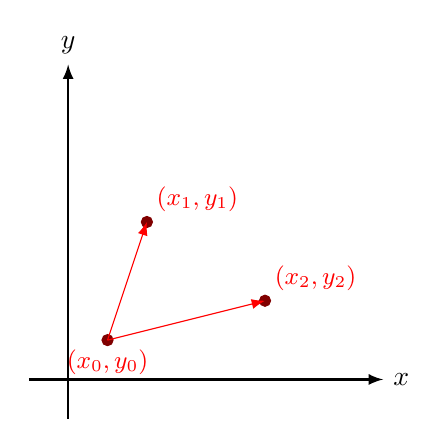
\begin{tikzpicture}
            \draw[thick,-latex] (0,-0.5) -- (0,4) node[above]{$y$};
            \draw[thick,-latex] (-0.5,0) -- (4,0) node[right]{$x$};

            \filldraw[red!50!black] (0.5,0.5) circle (2pt);
            \filldraw[red!50!black] (1,2) circle (2pt);
            \draw[red,-Latex] (0.5,0.5) node[below]{\small$(x_0,y_0)$} -- (1,2) node[above right]{\small$(x_1,y_1)$};
            \filldraw[red!50!black] (2.5,1) circle (2pt);
            \draw[red,-Latex] (0.5,0.5) -- (2.5,1) node[above right]{\small$(x_2,y_2)$};
        \end{tikzpicture}
        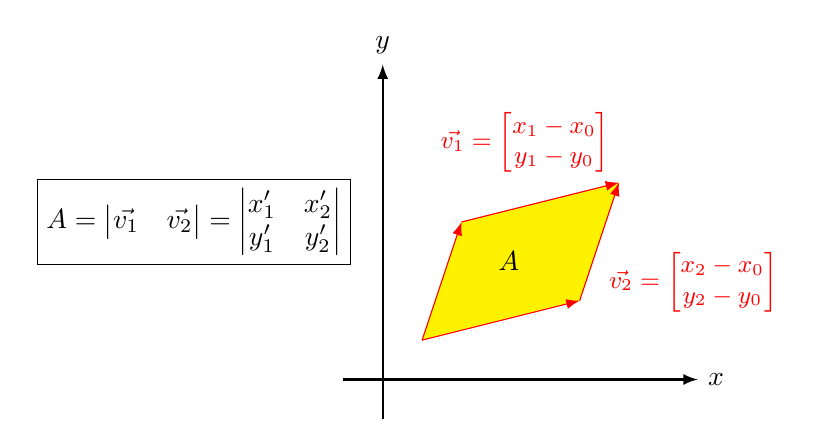
\begin{tikzpicture}
            \draw[thick,-latex] (0,-0.5) -- (0,4) node[above]{$y$};
            \draw[thick,-latex] (-0.5,0) -- (4,0) node[right]{$x$};

            \fill[yellow] (0.5,0.5) -- (1,2) -- (3,2.5) -- (2.5,1) -- cycle;
            \node at (1.6,1.5) {$A$};

            \draw[red,-Latex] (0.5,0.5) -- (1,2);
            \draw[red,-Latex] (0.5,0.5) -- (2.5,1);
            \draw[red,-Latex] (1,2) -- (3,2.5) node[above left]{\small$\vec{v_1}=\begin{bmatrix} x_1-x_0\\y_1-y_0 \end{bmatrix}$};
            \draw[red,-Latex] (2.5,1) -- (3,2.5) node[midway, below right]{\small$\vec{v_2}=\begin{bmatrix} x_2-x_0\\y_2-y_0 \end{bmatrix}$};

            \node at (-2.4,2) {$\boxed{A =\begin{vmatrix} \vec{v_1} & \vec{v_2} \end{vmatrix}=\begin{vmatrix} x_1' & x_2'\\y_1' & y_2' \end{vmatrix}}$};
        \end{tikzpicture}
        \end{center}
        Now divide the parallelogram into two triangle such that we get the area of triangle is half of the area of parallelogram.
        \begin{center}
            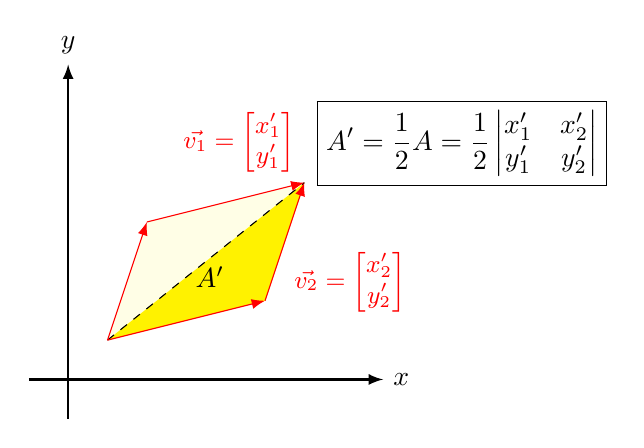
\begin{tikzpicture}
                \draw[thick,-latex] (0,-0.5) -- (0,4) node[above]{$y$};
                \draw[thick,-latex] (-0.5,0) -- (4,0) node[right]{$x$};

                \fill[yellow!10] (0.5,0.5) -- (1,2) -- (3,2.5) -- (2.5,1) -- cycle;
                \fill[yellow] (0.5,0.5) -- (3,2.5) -- (2.5,1) -- cycle;
                \draw[dashed] (0.5,0.5) -- (3,2.5);
                \node at (1.8,1.3) {$A'$};

                \draw[red,-Latex] (0.5,0.5) -- (1,2);
                \draw[red,-Latex] (0.5,0.5) -- (2.5,1);
                \draw[red,-Latex] (1,2) -- (3,2.5) node[above left]{\small$\vec{v_1}=\begin{bmatrix} x_1'\\y_1' \end{bmatrix}$};
                \draw[red,-Latex] (2.5,1) -- (3,2.5) node[midway, below right]{\small$\vec{v_2}=\begin{bmatrix} x_2'\\y_2' \end{bmatrix}$};

                \node at (5,3) {$\boxed{A' =\dfrac{1}{2}A=\dfrac{1}{2}\begin{vmatrix} x_1' & x_2'\\y_1' & y_2' \end{vmatrix}}$};
            \end{tikzpicture}
        \end{center}
        The area of a convex polygon can be calculated by summing the area of all triangles formed by the first point and two consecutive points. The illustration is shown below:
        \begin{center}
            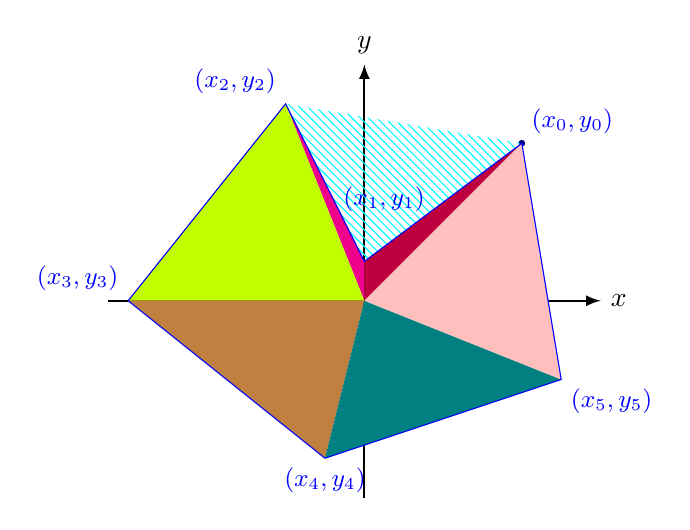
\begin{tikzpicture}[scale=0.5]
                \draw[thick,-latex] (0,-5) -- (0,6) node[above]{$y$};
                \draw[thick,-latex] (-6.5,0) -- (6,0) node[right]{$x$};

                \filldraw[blue!50!black] (4,4) circle (2pt);
                \fill[pattern=north west lines,pattern color=cyan] (4,4) -- (0,1) -- (-2,5) -- cycle;
                \fill[purple] (0,0)--(4,4) -- (0,1)-- cycle;
                \fill[magenta] (0,0) -- (0,1) -- (-2,5) -- cycle;
                \fill[lime] (0,0) -- (-2,5) -- (-6,0) -- cycle;
                \fill[brown] (0,0) -- (-6,0) -- (-1,-4) -- cycle;
                \fill[teal] (0,0) -- (-1,-4) -- (5,-2) -- cycle;
                \fill[pink] (0,0) -- (5,-2) -- (4,4) -- cycle;
                \node[above ,blue] at (0.5,2) {\small$(x_1,y_1)$};
                \draw[blue] (4,4) node[above right]{\small$(x_0,y_0)$} -- (0,1) -- (-2,5) node[above left]{\small$(x_2,y_2)$}-- (-6,0) node[above left]{\small$(x_3,y_3)$}-- (-1,-4) node[below]{\small$(x_4,y_4)$}-- (5,-2) node[below right]{\small$(x_5,y_5)$}-- cycle;
            \end{tikzpicture}
        \end{center}
        In previous illustration, we can see that the area of the polygon is the sum of the area of all triangles. If the polygon isn't convex, we can count the area like cyan triangle and sum the area of all triangles.
        We can generalize the formula for the area of a triangle with the following formula:
        \begin{equation*}
            A = \dfrac{1}{2}\sum_{k=1}^{n}\begin{vmatrix}
                x_{k-1} & x_{(k\mod n)}\\
                y_{k-1} & y_{(k\mod n)}
            \end{vmatrix}
        \end{equation*}
        The program can be implemented as follows:
        \begin{lstlisting}[backgroundcolor=\color{bg}]
package Aplro2.Week14;

import java.util.ArrayList;
import java.util.Scanner;

public class Liang_Ch11_15 {
    public static double DetArea2D(ArrayList<Double> vec1, ArrayList<Double> vec2) {
        return vec1.get(0) * vec2.get(1) - vec1.get(1) * vec2.get(0);
    }
    public static ArrayList<Double> Vector(ArrayList<Double> origin, ArrayList<Double> end) {
        ArrayList<Double> vector = new ArrayList<>();
        vector.add(end.get(0) - origin.get(0));
        vector.add(end.get(1) - origin.get(1));
        return vector;
    }
    public static ArrayList<ArrayList<Double>> InputPoints(int n){
        ArrayList<ArrayList<Double>> points = new ArrayList<>();
        try (Scanner input = new Scanner(System.in)) {
            for (int i = 0; i < n; i++) {
                ArrayList<Double> innerList = new ArrayList<>();
                for (int j = 0; j < 2; j++) {
                    innerList.add(input.nextDouble());
                }
                points.add(innerList);
            }
        }
        return points;
    }
    public static double AreaPolygon(ArrayList<ArrayList<Double>> points) {
        double area = 0;
        for (int i = 1; i < points.size()-1; i++) {
            ArrayList<Double> vec1 = Vector(points.get(0), points.get(i));
            ArrayList<Double> vec2 = Vector(points.get(0), points.get(i + 1));
            area += Math.abs(DetArea2D(vec1, vec2));
        }
        return area / 2;
    }
}
        \end{lstlisting}
        Some explanation about the code above:
        \begin{itemize}
            \item \texttt{DetArea2D} method is used to calculate the determinant of a $2\times 2$ matrix.
            \item \texttt{Vector} method is used to calculate the vector between two points.
            \item \texttt{InputPoints} method is used to input the points of the polygon.
            \item \texttt{AreaPolygon} method is used to calculate the area of the polygon.
        \end{itemize}
        Eventually, we create the main program as follows:
        \begin{lstlisting}[backgroundcolor=\color{bg}]
package Aplro2.Week14;
import java.util.Scanner;

public class CheckMethod extends Liang_Ch11_15{
    public static void main(String[] args) {
        try (Scanner input = new Scanner(System.in)) {
            System.out.print("Enter the number of the points: ");
            int n = input.nextInt();
            System.out.println("Enter the coordinates of the points: ");
            System.out.println("Total area is: " + AreaPolygon(InputPoints(n)));
        }
    }
}
        \end{lstlisting}
        Here is another sample run of the program:
        \begin{lstlisting}[backgroundcolor=\color{vscode},basicstyle=\small\ttfamily\color{white}]
Enter the number of the points: (*\raisebox{0pt}[1pt]{\colorbox{darkgray}{6}}*) (*\enter*)
Enter the coordinates of the points:
(*\raisebox{0pt}[1pt]{\colorbox{darkgray}{4 4 5 -2 -1 -4 -6 0 -2 5 0 1}}*) (*\enter*)
Total area is: 77.0
        \end{lstlisting}
        \item[\color{lblue}11.16] (\textit{Addition quiz}) Rewrite Listing 5.1 RepeatAdditionQuiz.java to alert the user if an answer is entered again. \textit{Hint: Use an array list to store answers.} Here is a sample run:
        \begin{lstlisting}
What is 5 + 9? (*\nextline{12}*) (*\enter*)
Wrong answer. Try again. What is 5 + 9? (*\nextline{34}*) (*\enter*)
Wrong answer. Try again. What is 5 + 9? (*\nextline{12}*) (*\enter*)
You already entered 12
Wrong answer. Try again. What is 5 + 9? (*\nextline{14}*) (*\enter*)
You got it!
        \end{lstlisting}
        \jawab\\
        The program can be implemented as follows:
        \begin{lstlisting}[backgroundcolor=\color{bg}]
package Aplro2.Week14;

import java.util.ArrayList;
import java.util.Scanner;

public class Liang_Ch11_16 {
    public static void main(String[] args) {
        try (Scanner input = new Scanner(System.in)) {
            int number1 = (int) (Math.random() * 10);
            int number2 = (int) (Math.random() * 10);
            int answer;
            ArrayList<Integer> answers = new ArrayList<>();

            System.out.print("What is " + number1 + " + " + number2 + "? ");
            answer = input.nextInt();

            while (answer != number1 + number2) {
        \end{lstlisting}
        \begin{lstlisting}[backgroundcolor=\color{bg}]
                if (answers.contains(answer)) {
                    System.out.println("You already entered " + answer);
                } else {
                    System.out.println("Wrong answer. Try again.");
                    answers.add(answer);
                }
                System.out.print("What is " + number1 + " + " + number2 + "? ");
                answer = input.nextInt();
            }
        }
        System.out.println("You got it!");
    }
}
        \end{lstlisting}
        Then we can run the program. Here is a sample run of the program:
        \begin{lstlisting}[backgroundcolor=\color{vscode},basicstyle=\small\ttfamily\color{white}]
What is 7 + 8? (*\raisebox{0pt}[1pt]{\colorbox{darkgray}{9}}*) (*\enter*)
Wrong answer. Try again.
What is 7 + 8? (*\raisebox{0pt}[1pt]{\colorbox{darkgray}{0}}*) (*\enter*)
Wrong answer. Try again.
What is 7 + 8? (*\raisebox{0pt}[1pt]{\colorbox{darkgray}{9}}*) (*\enter*)
You already entered 9
What is 7 + 8? (*\raisebox{0pt}[1pt]{\colorbox{darkgray}{0}}*) (*\enter*)
You already entered 0
What is 7 + 8? (*\raisebox{0pt}[1pt]{\colorbox{darkgray}{15}}*) (*\enter*)
You got it!
        \end{lstlisting}
    \end{enumerate}
\end{document}